\subsection{ELBO}
Evidence lower bound
$$\mathbb{E}[\log{p_\theta(x|z)}] - \mathbb{E}[\log{\frac{q_\phi(z|x)}{p_\theta(z)}}]$$

\begin{figure}[h]
    \centering
    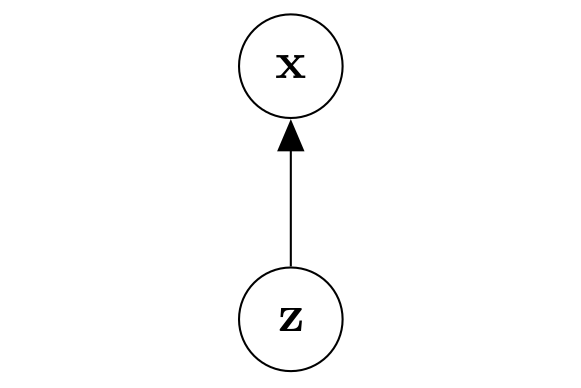
\includegraphics[width=0.2\textwidth]{images/latent_variable_mode.png}
    \caption{Latent variable model}
    \label{fig:lanent_variable_model}
\end{figure}

Latent variable model (Fig. \ref{fig:lanent_variable_model}) and bayes rule to obtain the posterior distribution:
Posterior $p_\theta(z|x)$, likelihodd $p_\theta(x|z)$, prior $p_\theta(z)$, normalizing constant (evidence) $p_\theta(x)$,

$$p_\theta(z|x) = \frac{p_\theta(x|z)p_\theta(z)}{p_\theta(x)}$$

Approximate the \textbf{posterior} with another distribution $q_\phi(z|x)$.
So our goal is defined $p_\theta(z|x)\approx q_\phi(z|x)$.
That is simply to approximate the intactable posterior distribution with a simpler distribution.
But we still have to learn parameters $\phi$ using optimization.
Optimization requires a loss function.
We need to predict the similarity between two probability distributions $p$ and $q$.
So we need KL-divergence $D_{KL}(p_\theta|q_\phi)$. Let's calculate reserve KL.

$$D_{KL}(q_\phi|p_\theta) = \mathbb{E}_{q_\phi}[\log{\frac{q_\phi(z|x)}{p_\theta(z|x)}}]$$

We need to minimize it, but we have trouble with denominator $p_\theta(z|x)$ which we want to approximate.

\begin{equation}
    \begin{aligned}
        \text{KL} \big( q(\mathbf{z}) || p(\mathbf{z} | \mathbf{x}) \big)
         & = \int q(\mathbf{z}) \log \frac{q(\mathbf{z})}{p(\mathbf{z} | \mathbf{x})} d\mathbf{z}                                                  & \text{(1.1)} \\
         & = \int q(\mathbf{z}) \big( \log q(\mathbf{z}) - \log p(\mathbf{z} | \mathbf{x}) \big) d\mathbf{z}                                       & \text{(1.2)} \\
         & = \int q(\mathbf{z}) \log q(\mathbf{z}) - q(\mathbf{z}) \log p(\mathbf{z} | \mathbf{x}) d\mathbf{z}                                     & \text{(1.3)} \\
         & = \int q(\mathbf{z}) \log q(\mathbf{z}) d\mathbf{z} - \int q(\mathbf{z}) \log p(\mathbf{z} | \mathbf{x}) d\mathbf{z}                    & \text{(1.4)} \\
         & = \mathbb{E}_{q} \big[ \log q(\mathbf{z}) \big] - \mathbb{E}_{q} \big[ \log p(\mathbf{z} | \mathbf{x}) \big]                            & \text{(1.5)} \\
         & = \mathbb{E}_{q} \big[ \log q(\mathbf{z}) \big] - \mathbb{E}_{q} \bigg[ \log \frac{p(\mathbf{x}, \mathbf{z}) }{p(\mathbf{x})} \bigg]    & \text{(1.6)} \\
         & = \mathbb{E}_{q} \big[ \log q(\mathbf{z}) \big] - \mathbb{E}_{q} \big[ \log p(\mathbf{x}, \mathbf{z}) - \log p(\mathbf{x}) \big]        & \text{(1.7)} \\
         & = \mathbb{E}_{q} \big[ \log q(\mathbf{z}) - \log p(\mathbf{x}, \mathbf{z}) \big] + \mathbb{E}_{q} \big[ \log p(\mathbf{x}) \big]        & \text{(1.8)} \\
         & = \mathbb{E}_{q} \big[ \log q(\mathbf{z}) - \log p(\mathbf{x}, \mathbf{z}) \big] + \underbrace{\log p(\mathbf{x})}_{\text{intractable}} & \text{(1.9)} \\
    \end{aligned}
\end{equation}
\footnotetext{\url{https://mpatacchiola.github.io/blog/2021/01/25/intro-variational-inference.html}}

$\log{p_\theta(x)}$ - marginal log likelihood (Log evidence)

\begin{equation}
    \mathbb{E}_{q} \big[\log p(\mathbf{x}, \mathbf{z}) - \log q(\mathbf{z}) \big] = \log p(\mathbf{x}) - \text{KL} \big( q(\mathbf{z}) || p(\mathbf{z} | \mathbf{x}) \big)
\end{equation}

As $KL \geq 0$

\begin{equation}
    \mathbb{E}_{q} \big[\log p(\mathbf{x}, \mathbf{z}) - \log q(\mathbf{z}) \big] \leq \log p(\mathbf{x})
\end{equation}

The left part called evidence lower bound

\begin{equation}
    \begin{aligned}
        \mathrm{ELBO}(q)
         & =\mathbb{E}_{q} \big[\log p(\mathbf{x}, \mathbf{z}) - \log q(\mathbf{z}) \big]                                                 & \text{(2.1)} \\
         & =\mathbb{E}_{q}[\log p(\mathbf{z}, \mathbf{x})] -\mathbb{E}_{q}[\log q(\mathbf{z})]                                            & \text{(2.2)} \\
         & =\mathbb{E}_{q}[\log \big( p(\mathbf{x} \vert \mathbf{z}) p(\mathbf{z}) \big) ] -\mathbb{E}_{q}[\log q(\mathbf{z})]            & \text{(2.3)} \\
         & =\mathbb{E}_{q}[\log p(\mathbf{x} \vert \mathbf{z})] + \mathbb{E}_{q}[\log p(\mathbf{z})] - \mathbb{E}_{q}[\log q(\mathbf{z})] & \text{(2.4)} \\
         & =\mathbb{E}_{q}[\log p(\mathbf{x} \vert\mathbf{z})] + \mathbb{E}_{q}[\log p(\mathbf{z}) - \log q(\mathbf{z})]                  & \text{(2.5)} \\
         & =\mathbb{E}_{q}[\log p(\mathbf{x} \vert \mathbf{z})] + \int q(\mathbf{z}) \log \frac{p(\mathbf{z})}{q(\mathbf{z})} d\mathbf{z} & \text{(2.6)} \\
         & =\mathbb{E}_{q}[\log p(\mathbf{x} \vert \mathbf{z})]- \text{KL}(q(\mathbf{z}) \| p(\mathbf{z}))                                & \text{(2.7)}
    \end{aligned}
\end{equation}

\subsection{CLIP}
\begin{figure}[h]
    \centering
    \includegraphics[width=1\textwidth]{images/main-diagrams.pdf}
    \caption{CLIP architecture}
    \label{fig:clip_main_diagram}
\end{figure}

How do we connect images with text. What if we have dataset of image-text pairs.
This kind of images you can find on the Internet, so it's relatively easy to get that kind of dataset.
If we can somehow learn to connect images with text. We won't be bound with the labels for classification.
We will get very good representation.

So how it works. We are going to take an image, pass it through encoder.
It gives us image representation, vector in latent space. We will do it in batches $I_1, ..., I_n$ (Fig. \ref{fig:clip_main_diagram}).
We also obtain a vector representation for text $T_1, ..., T_n$.
In the training set we know that $I_1$ goes with $T_1$ and so on, because we scape dataset in that way.

Previously we try to predict image with text. So we take an image vector and try to predict the text.
We no longer do that. We are simply ask the model for this representation which of these texts are the most appropriate.
So that's an constractive objective. We fit an image and ask it which of all these texts are the closest.
You see that it heavily relies on batch size.

On inference. You take an image, put it through image encoder and get image representation model.
You get all labels of classification task. You engineer a prompt. You encode all labels with prompt context through text encoder.
You simply ask wich of this labels is the closest, so the inner product is the hightest.
Zero training needed  (\cite{radford2021learning}).
\subsection{Diffusion Models}
Diffusion model is different type of generative model.
GAN basically is a neural network with bunch layers. You sample some noise, you get the noise vector $z$.
You put the $z$ through the network and it gives you a picture. You train network using discriminator to produce pictures.
So the mapping is noise to picture.

In diffusion models it's the reverse. You take an image. You are going to put a noise on the image.
So you get a slightly noisy version of image. Then you do it again and again.
Your picture will get noiser and noiser. What comes at the end is just a noirmaly distributed noise.
However every step is very small. Technicaly it's possible for the model to look a slightly noised image and predict the sharp version.
The individual step is small enough, so the model can reconstruct it.
However if we do it long enough we are adding standart normal distribution.
So we can sample some noise from standart distribution. Put it throught the process of reconstruction.

\begin{figure}[h]
    \centering
    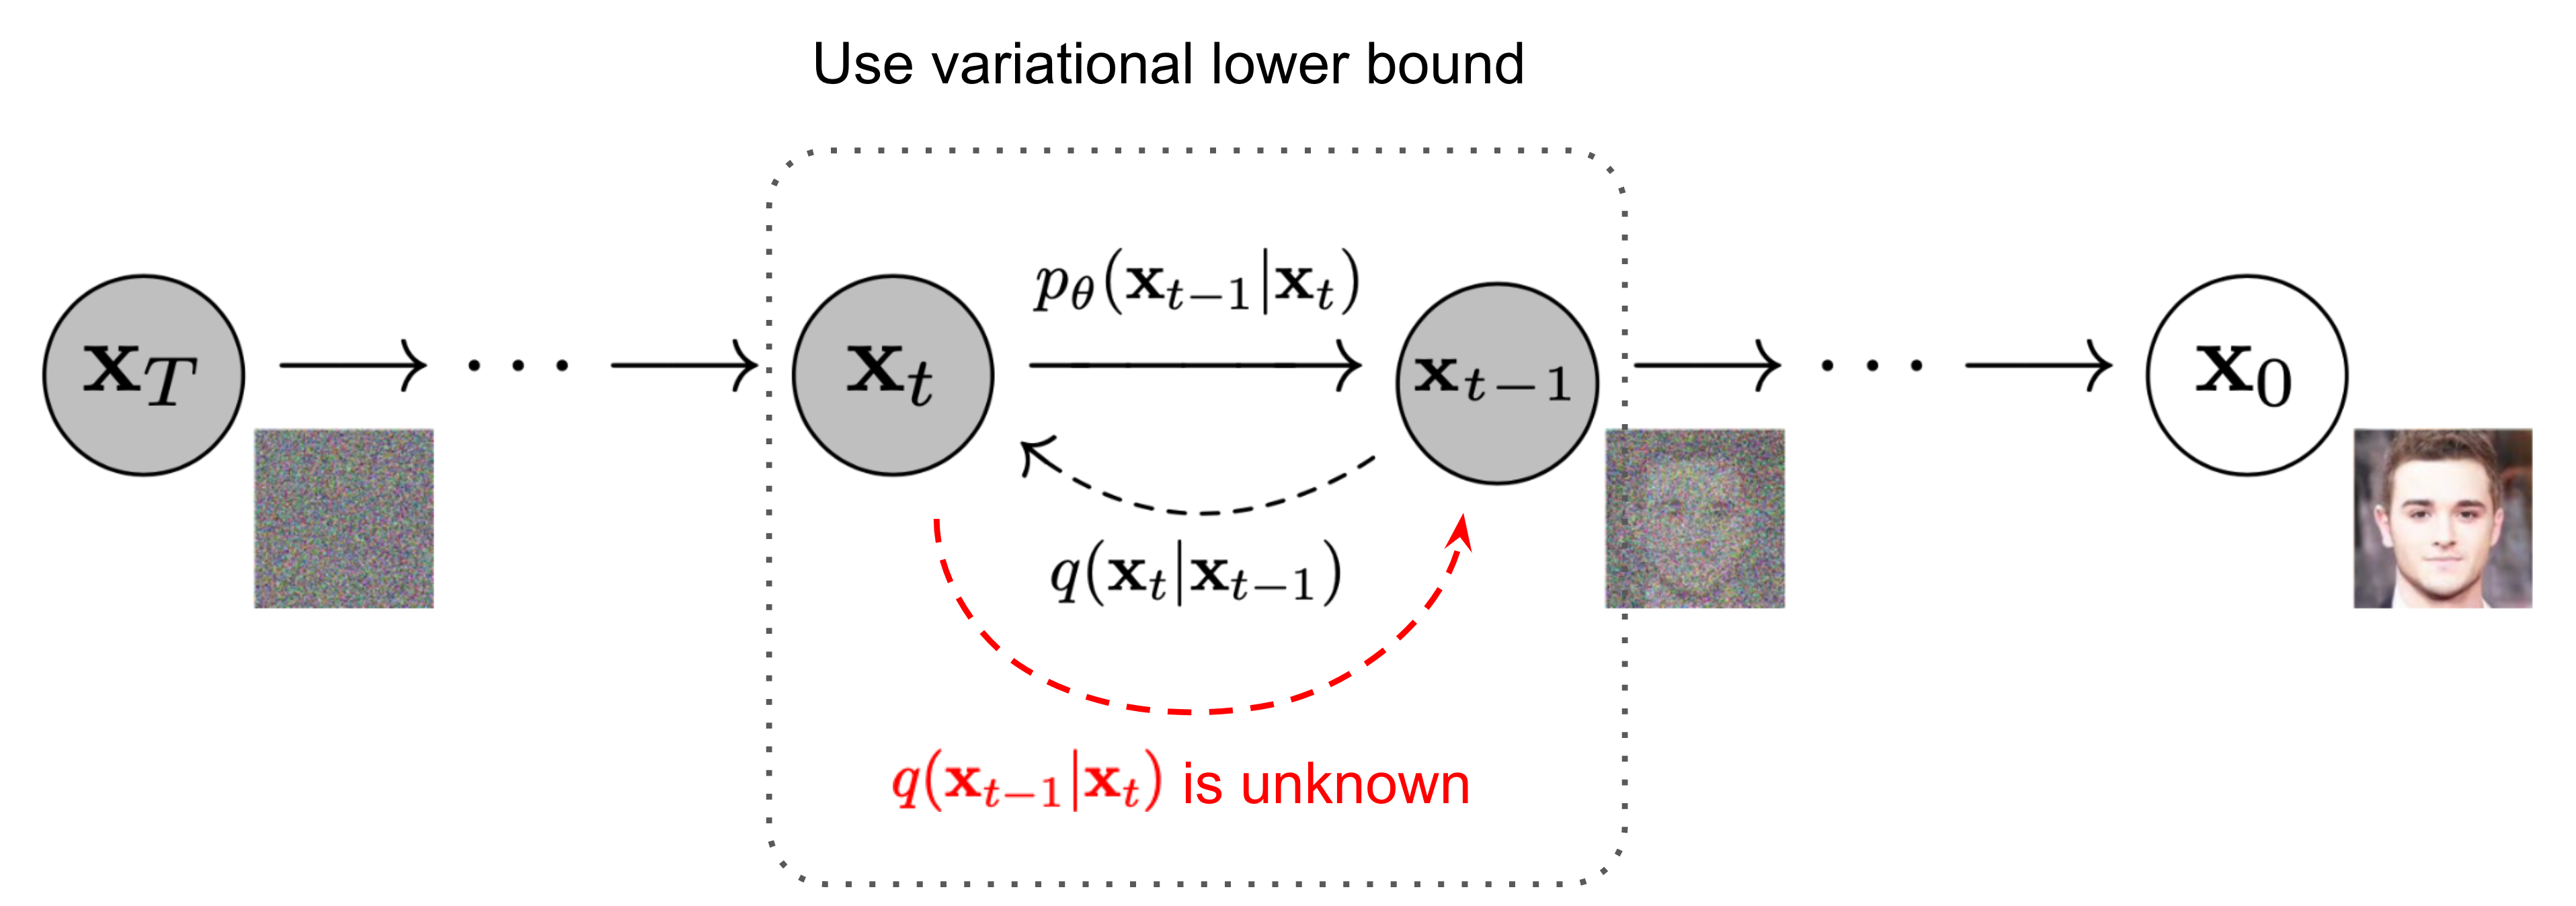
\includegraphics[width=1\textwidth]{images/ddpm.png}
    \caption{Diffusion model}
    \label{fig:ddpm}
\end{figure}

Given a sample from the data distribution $x_0 \approx q(x_0)$. We produce a Markov chain of latent variables $x_1, ..., x_T$.
With $x_T$ finally be a normal distribution.

$$q(x_t|x_{t-1}) = \mathcal{N}(x_t; \sqrt{\alpha_t}x_{t-1}, (1-\alpha_t)\mathcal{I})$$
$$mean~vector = \sqrt{\alpha_t}x_{t-1}$$
$$covariance~matrix=(1-\alpha_t)\mathcal{I}$$

If the magnitute $1-\alpha_t$ of the noise added to each step is small enough,
the posterior $q(x_{t-1}|x_t)$ is well approximated by a diagonal Gaussian.
Furthermore, if the magnitute $1-\alpha_1...\alpha_t$ of the total noise is large enough,
$x_T$ is well approximated by $\mathcal{N}(0, \mathcal{I})$.
These properties suggest learning a model $p_\theta(x_{t-1}|x_t)$ to approximate true posterior.
So basically, we are going to train a neural net, which doesn't exactly going reconstruct the image,
but that's a variational model. So we are going to plug the $x_t$ to a neural net and it will give us mean and covariance matrix of the next step of the chain:

$$p_\theta(x_{t-1}|x_t)=\mathcal{N}(\mu_\theta(x_t), \Sigma_\theta(x_t))$$

So we start with the Gaussian noise $x_T=\mathcal{N}(0, \mathcal(I))$ and gradually reducing the noise in a sequence of steps $x_{T-1}, x_{T-2}, ..., x_0$ (\cite{ho2020denoising}).

Since we always adding Gaussian noise, we can add it in a one step. Rather then predicting image by itself, we are predicting noise $\epsilon=x_{t}-x_{t-1}$.
That is standart diffusion models.

\subsection{Guided diffusion models}
Next thing is guided diffusion models (\cite{nichol2021improved}). Their show a method to learn covariance matrix $\Sigma_\theta$.
Let's assume we have images and the class label. We can train neural net to predict noise, but we can also give it a label $y$.
So we train a class conditional model. It has some advantages. Class conditional models are fine, but we can do better. We could guide our model more.
One way to do that is to say I have a classifier. For example based on ImageNet. If I want to push my diffusion process toward a particular label.
I can take an ImageNet classifier and I can go along the gradient of that.

We can do CLIP guided diffusion process by taking $\nabla_{x_t} CLIP(x_t, text)$.
More formally, $\nabla_{x_t} log_{p_\phi}(y|x_t)$. You can push the diffusion process into the direction where the image would fit a text more because you go along gradient of that.
It's kind of constructing adversarial example towards this classifier.
$$\hat{\mu}_\theta(x_t|y)=\mu_\theta(x_t|y) + s * \Sigma_\theta(x_t|y) \nabla_{x_t}log_{p_\phi}(y|x_t)$$


But it means that you have to have an external classifier to go by. There is a method to do it without classifier called classifier free guidence.
The label $y$ in a class-conditional diffusion model $\epsilon_\theta(x_t, y)$ sometimes is replaced with a null label $\emptyset$:

$$\hat{\epsilon}_\theta(x_t|y) = \epsilon_\theta(x_t|\emptyset) + s * (\epsilon_\theta(x_t|y) - \epsilon_\theta(x_t|\emptyset))$$

Here, $s\geq1$ is the guidance scale.

\subsection{VQVAE}
What VAE do? It's parametrize the distribution. You have encoder, you output vector of means $\mu$ and vector of standard deviation $\sigma$.
You also want to do $log \sigma$ so we make sure standard deviation.
You sample a vector from that distribution and put it into the decoder. (\cite{oord2017neural})

\begin{figure}[h]
    \centering
    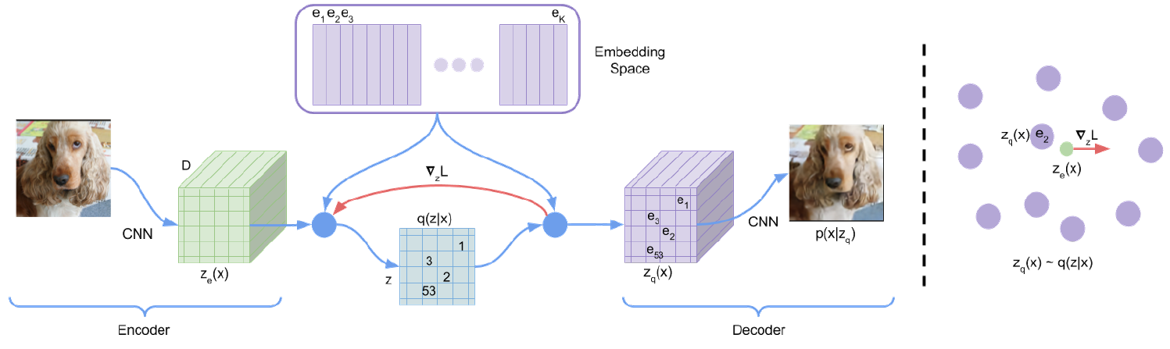
\includegraphics[width=0.5\textwidth]{images/vqvae.png}
    \caption{VQ-VAE}
    \label{fig:vq_vae}
\end{figure}

So how VQVAE works? We put image through encoder and get some representation. We take vectors and snap it onto distinct codebook (embedding space).
We want to find the closest one vectors and then map vectors from encoder and you put indexes into $q(z|x)$ matrix. And put only those into decoder.

How to backpropagate? Copy paste the gradients from decoder to encoder (marked with red arrow) (Fig. \ref{fig:vq_vae})

\subsection{VQVAE - 2}
Does the smae but in multiscale (Fig. \ref{fig:vq_vae2}).
\begin{figure}[h!]
    \centering
    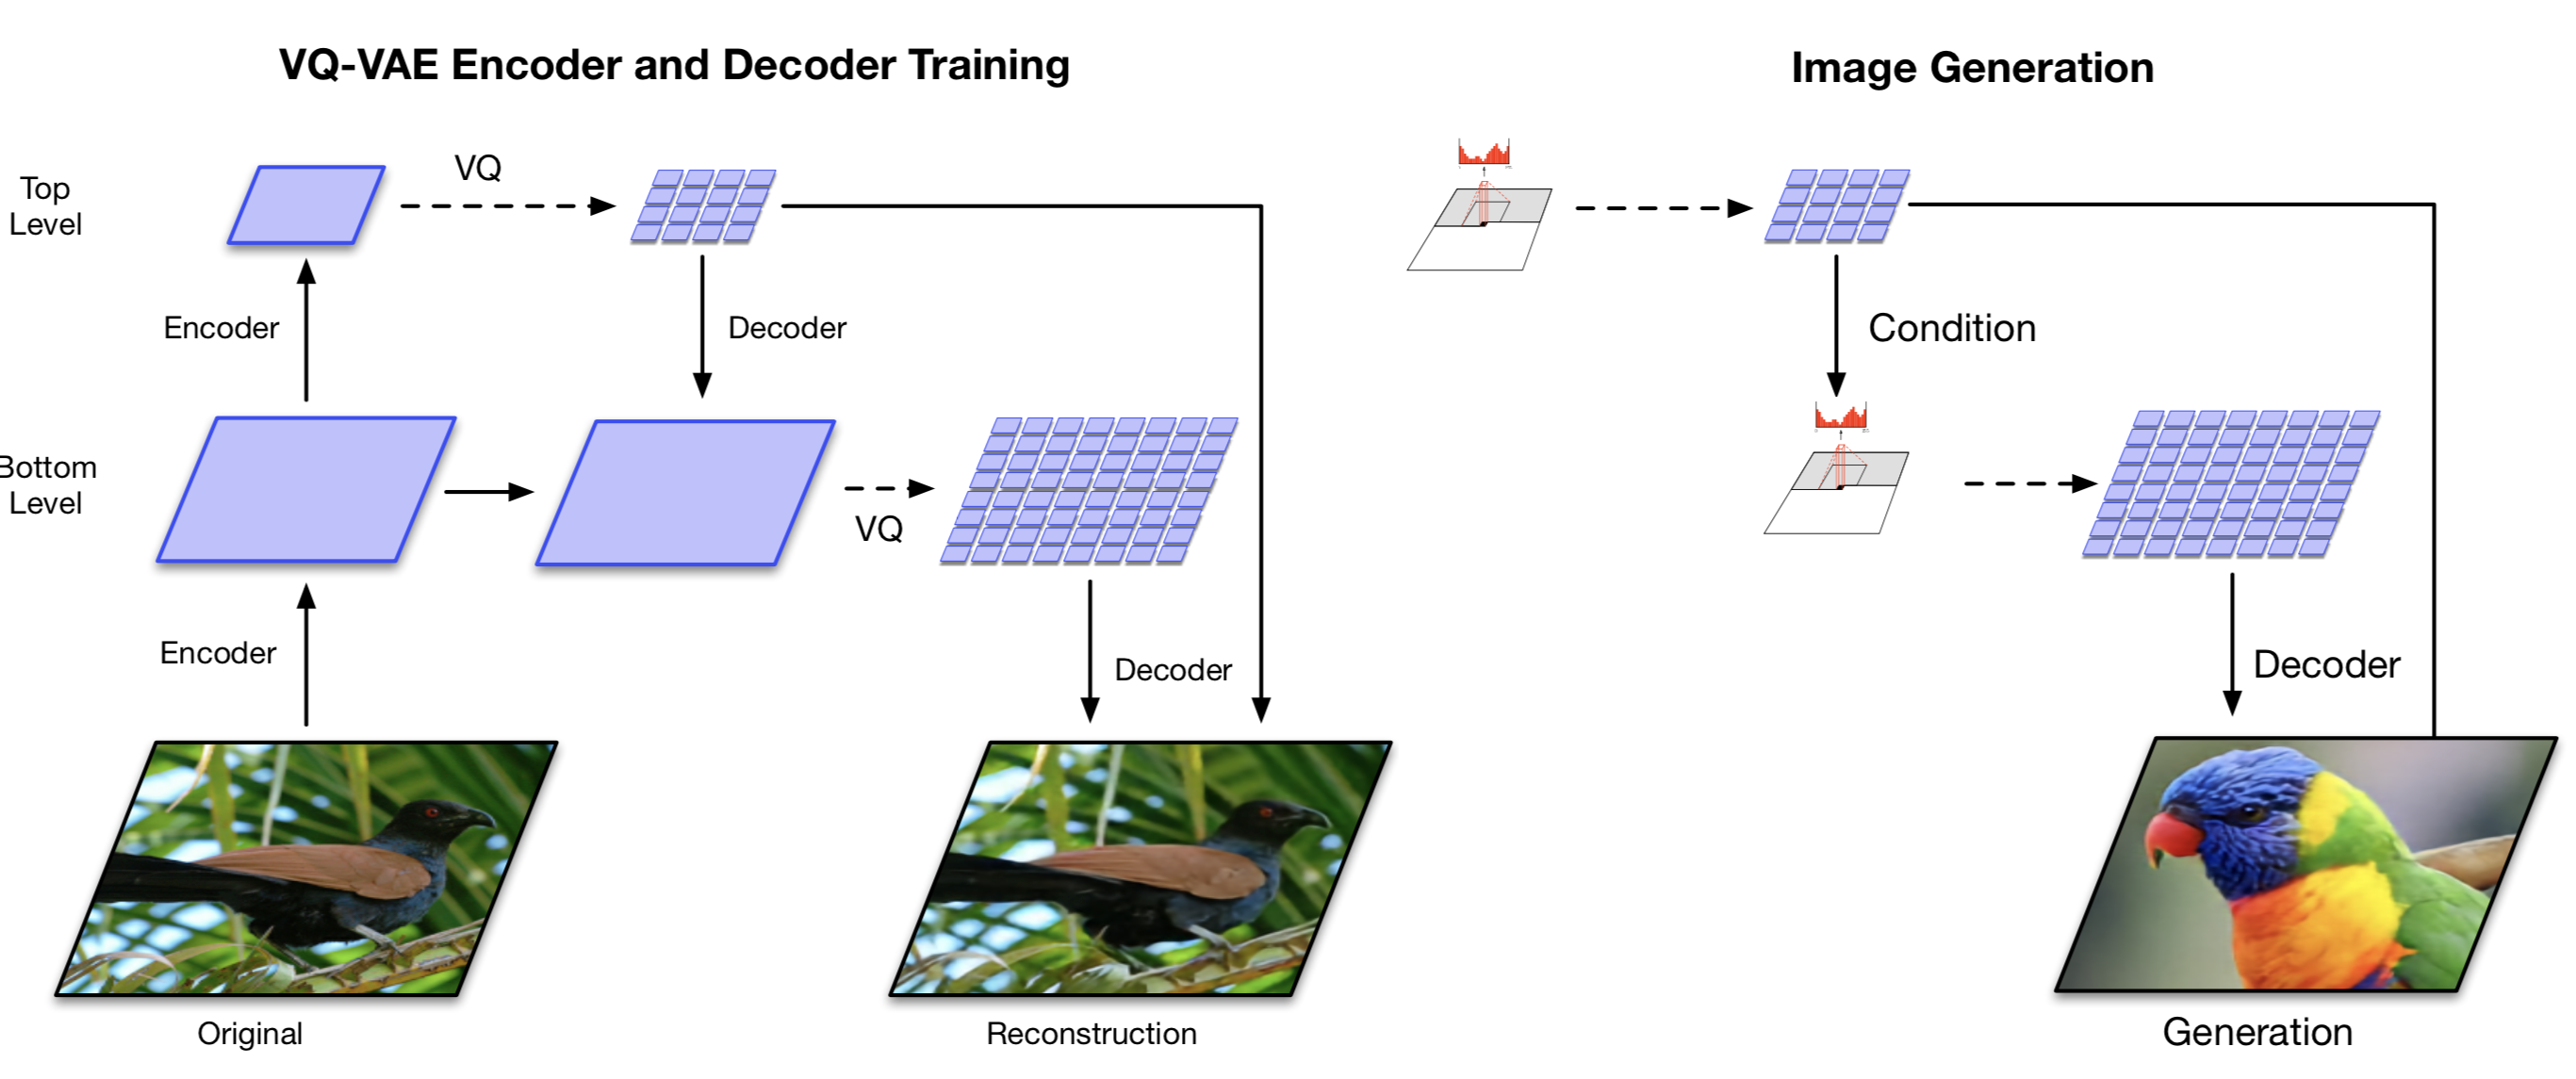
\includegraphics[width=0.5\textwidth]{images/vqvae2.png}
    \caption{VQ-VAE2}
    \label{fig:vq_vae2}
\end{figure}


\subsection{VQ-GAN}
\begin{figure}[h!]
    \centering
    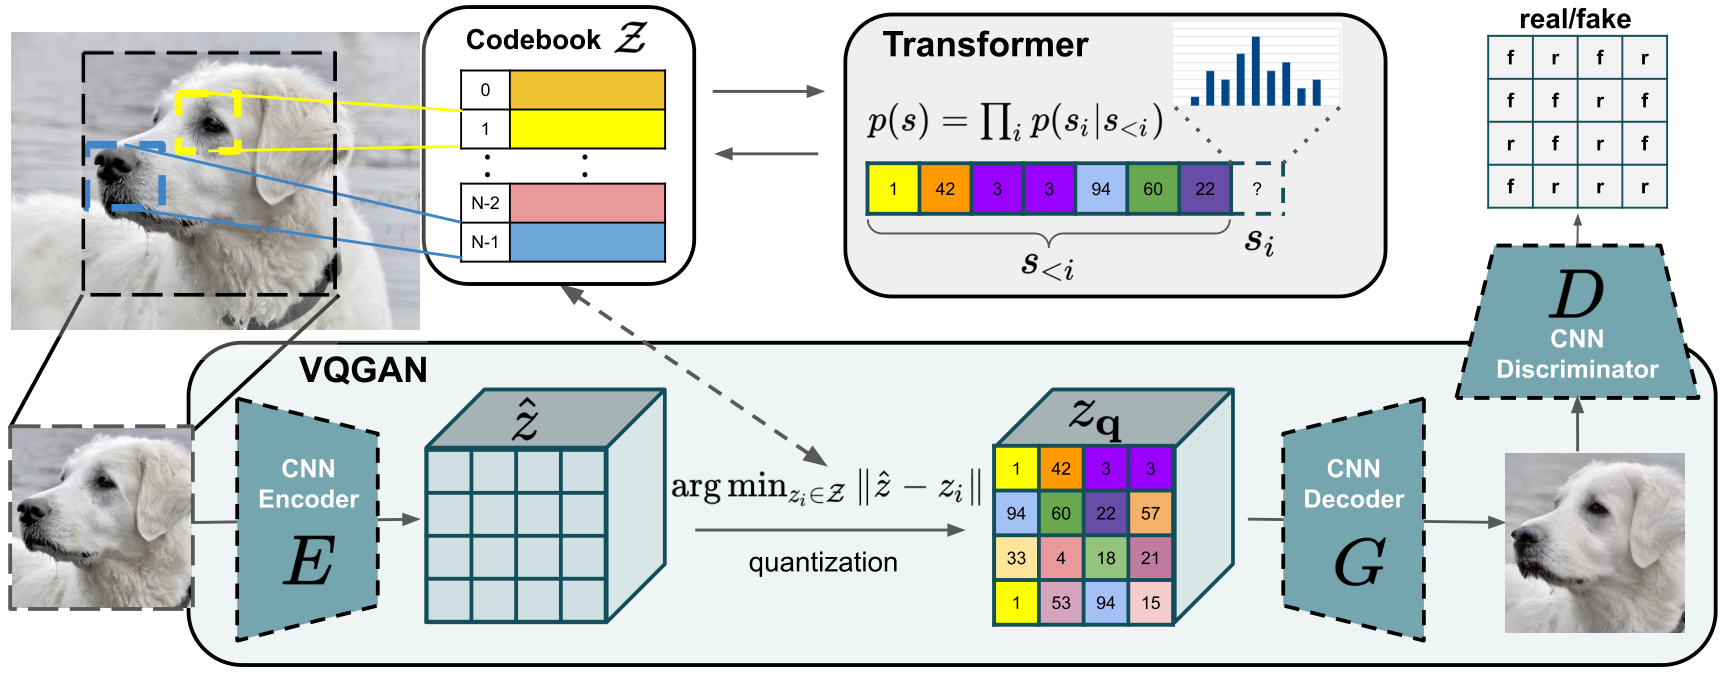
\includegraphics[width=0.5\textwidth]{images/vqgan.png}
    \caption{VQ-GAN}
    \label{fig:vq_gan}
\end{figure}
The encoder $E$, the decoder $G$ and the codebook $Z$ can be trained end-to-end via the following loss function \cite{esse2021vqgan}:


$$L_{VQVAE} = || x - \hat{x}||_1 + || sg[E(x)] -  z_q ||_2^2  + \beta || sg[z_q] - E(x)||_2^2$$

Where, $sg[\cdot ]$ stands for the stop-gradient operation.

\begin{itemize}
    \item Replaced L1/L2 loss with perceptual loss
    \item Added also adversarial loss
\end{itemize}


\subsection{VQ Diffusion Model (\cite{gu2021vector})}
\begin{figure}[h!]
    \centering
    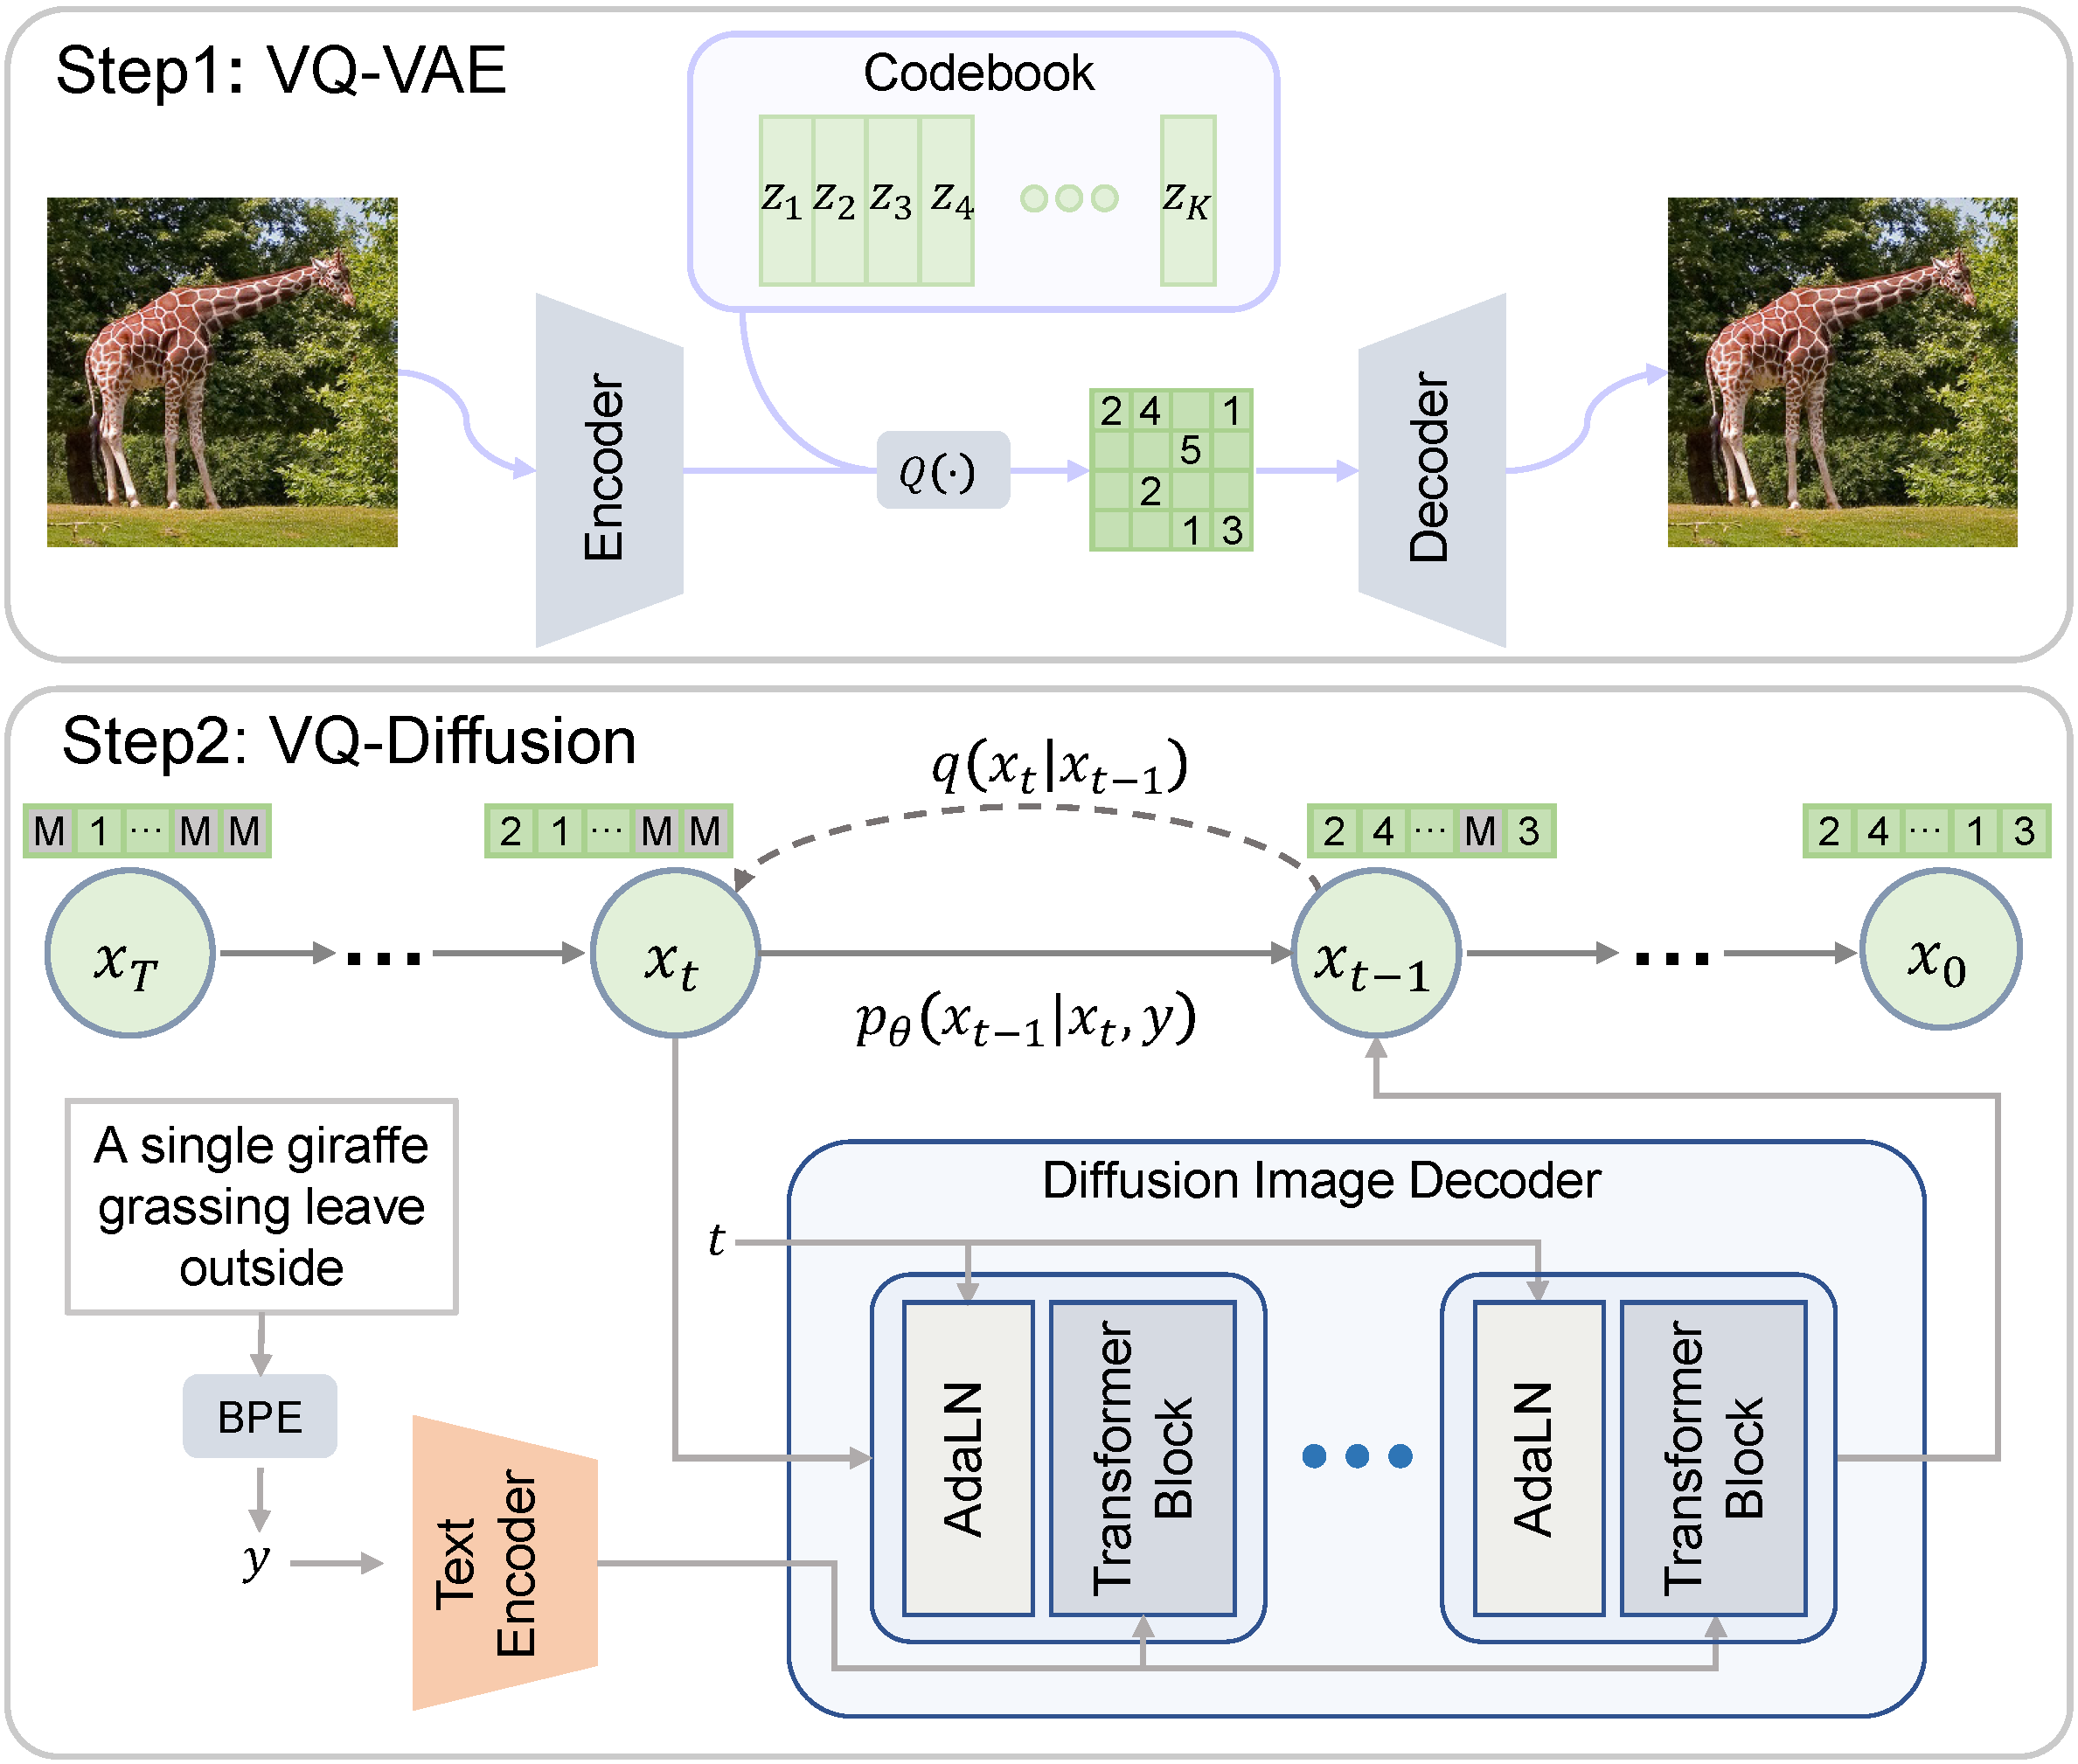
\includegraphics[width=0.5\textwidth]{images/vqddpm.png}
    \caption{VQ Diffusion model}
    \label{fig:vqddpm}
\end{figure}

\subsection{DiVAE (\cite{shi2022divae})}

DiVAE parametrizes $p(x|z)$ through a diffusion model
\begin{figure}[h!]
    \centering
    \includegraphics[width=0.5\textwidth]{images/divae.pdf}
    \caption{DiVAE}
    \label{fig:divae}
\end{figure}

\begin{figure}[h!]
    \centering
    \includegraphics[width=0.5\textwidth]{images/divae_architecture.pdf}
    \caption{DiVAE Architecture}
    \label{fig:divae_architecture}
\end{figure}


\subsection{DALL-E}
If we combine VQVAE with GPT-3 we get DALL-E (\cite{ramesh2021zeroshot})

\subsection{DALLE-2}
It works different than DALL-E. The main objective is CLIP.
DALLE-2 uses CLIP as a foundation for the generative model.
Previously CLIP was used as a ranker. They have a CLIP which is frozen and gives you text and image embeddings.
What DALLE-2 does is taking text embeddings and and there's two new parts.

The first one is a prior which can either be diffusion based or autoregressive based.
That prior is supposed to take the text embedding and make it into image embedding.
CLIP already tries to align the two quite well.
However, there's still a bit of a difference and that prior bridges that gap.
This could be trained in a supervised fasion.

The other new thing is a decoder which is a diffusion based model.
So that takes an image encoding and it forward propagates through a diffusion model (\cite{ramesh2022}).

\begin{figure}[h!]
    \centering
    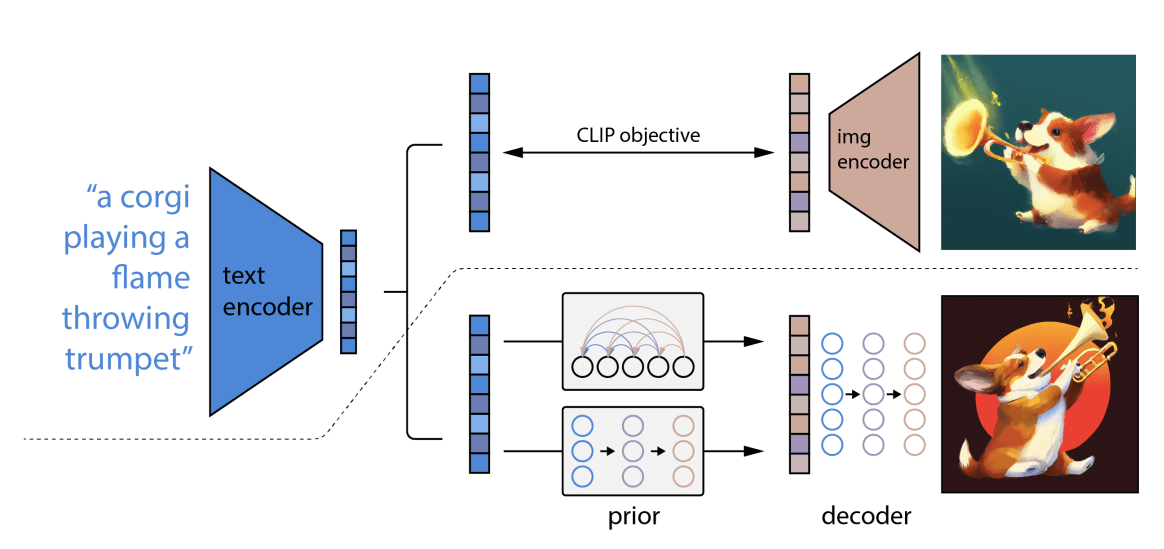
\includegraphics[width=0.5\textwidth]{images/dalle2.png}
    \caption{DALLE-2}
    \label{fig:dalle2}
\end{figure}

\subsection{Imagen}
They use huge text model. Instead of training a text model along with the image generation model.
They simply use big pre-trained model and freeze it so it doesn't change during the training of image generation model.
Now we need to use text embedding to generate image.
They use diffusion model to achive that (\cite{saharia2022photorealistic}).
Iteratively use super resolution models. First to upscale from 64x64 to 256x226. Then split into patches and upscale to 1024x1024 (Fig. \ref{fig:imagen})

\begin{figure}[h!]
    \centering
    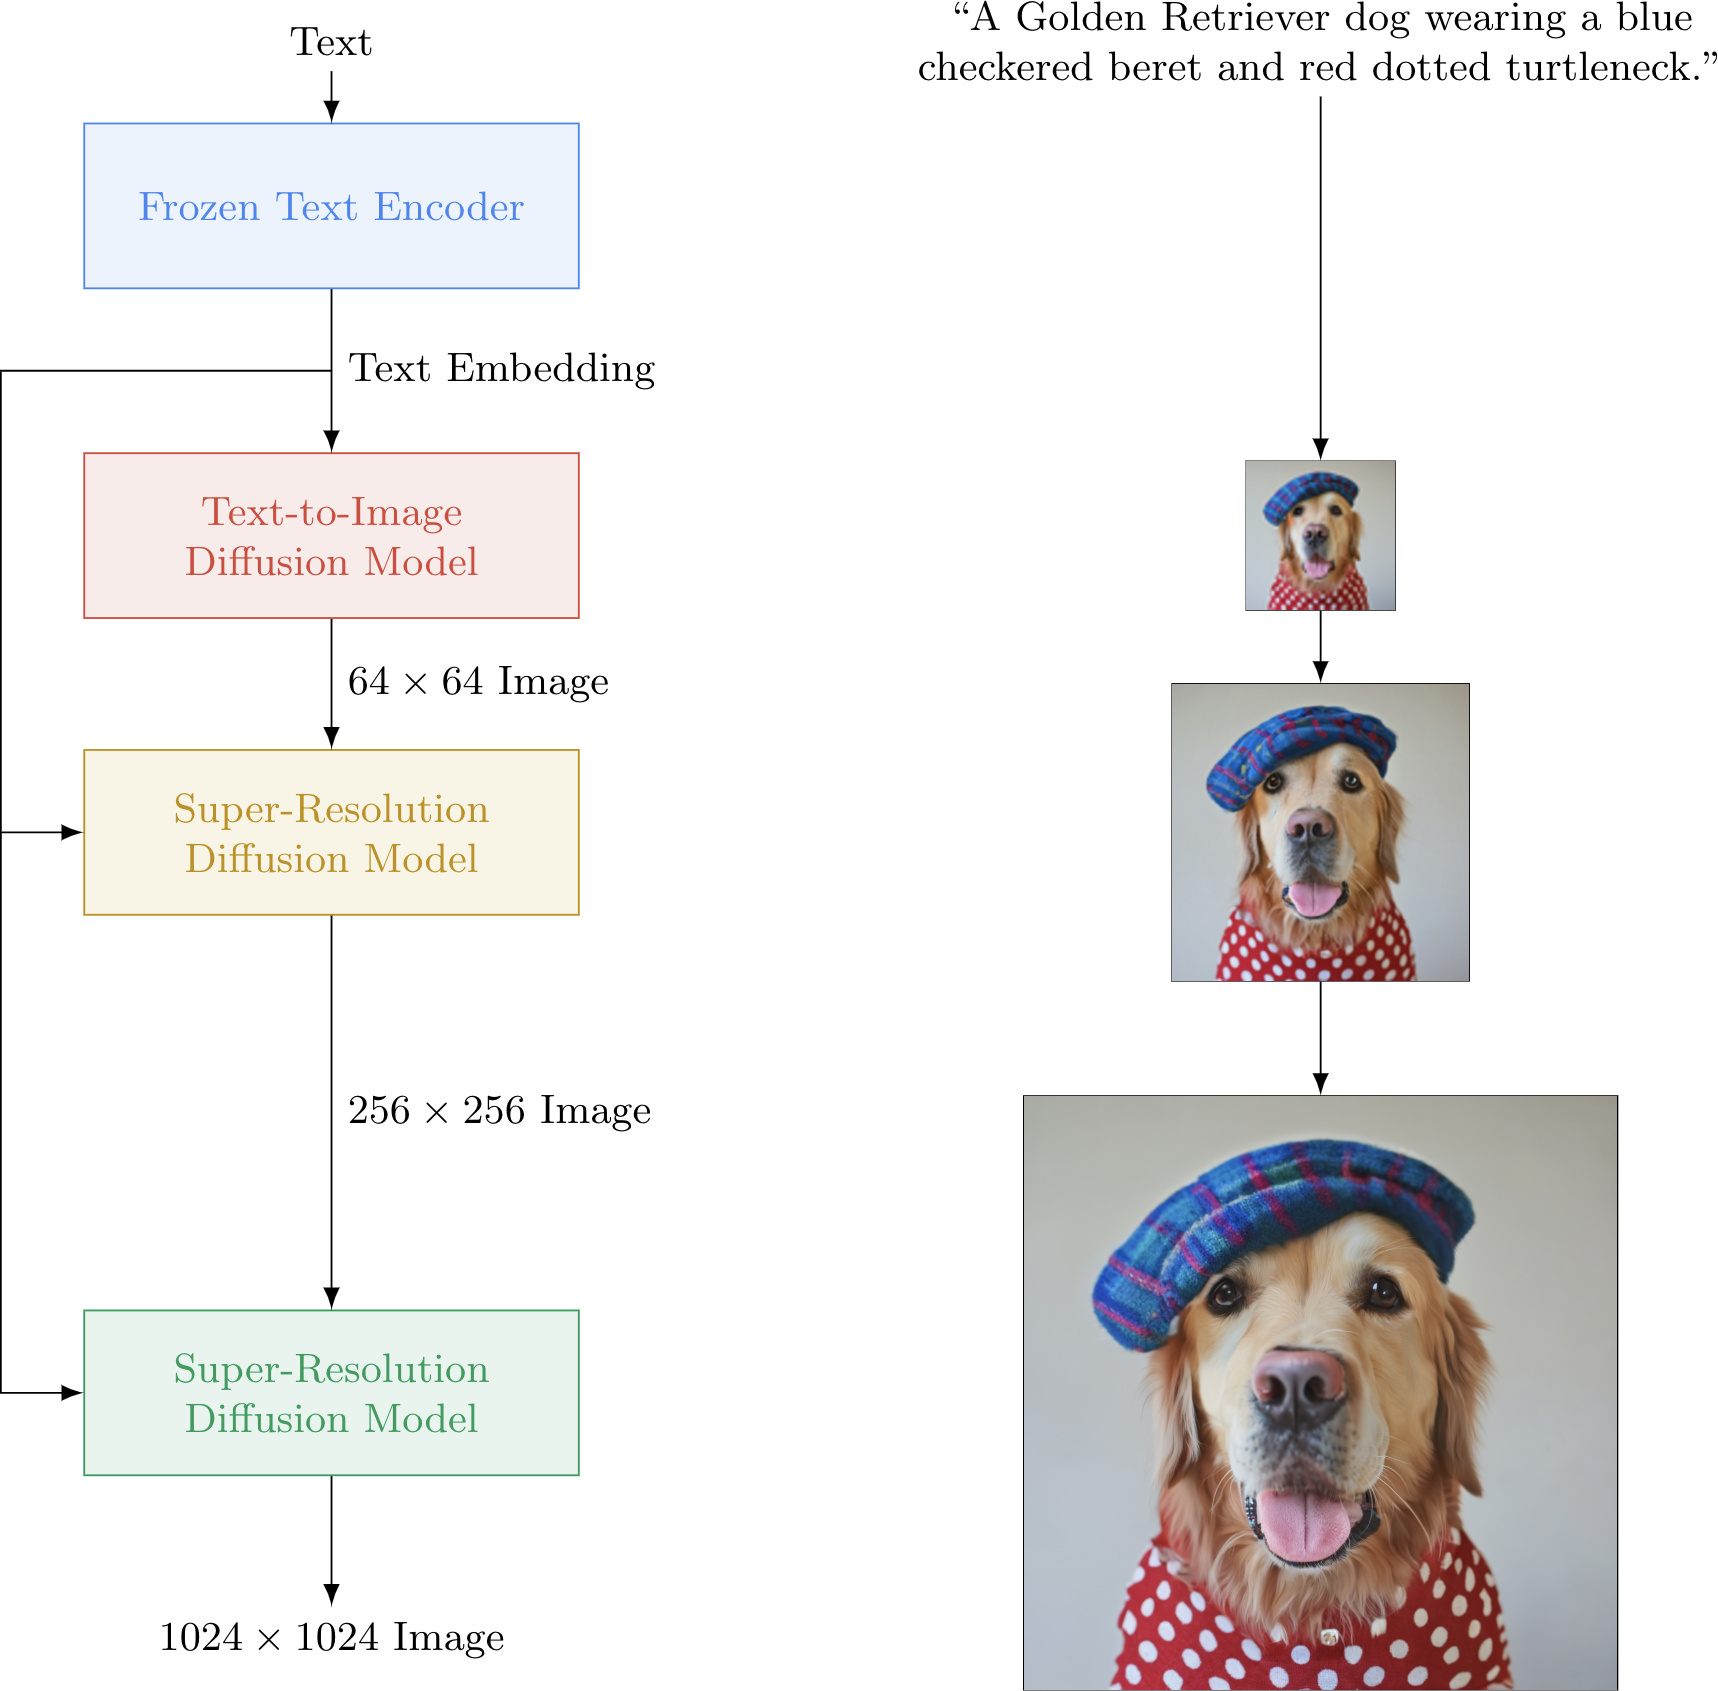
\includegraphics[width=0.5\textwidth]{images/imagen.jpg}
    \caption{Imagen}
    \label{fig:imagen}
\end{figure}
